\documentclass[../psets.tex]{subfiles}

\pagestyle{main}
\renewcommand{\leftmark}{Problem Set \thesection}
\setcounter{section}{2}

\begin{document}




\section{Peak Assignments}
\marginnote{3/6:}Darolutamide is an anti-androgen compound used in the treatment of prostate cancer in older men.
\begin{center}
    \footnotesize
    \chemfig{>:[6](-[:-30]\chembelow{N}{H}-[:30](=[2]O)-[:-30]*5(=N-NH-[,,1](-(-[::60]OH)-[::-60])=-))(-[:-150]-[:150]N*5(-=-(-*6(=-(-Cl)=(-~N)-=-))=N-))}
\end{center}
A single \SI{300}{\milli\gram} dose tablet weighs approximately \SI{610}{\milli\gram}. A sample of darolutamide was produced by crushing a single tablet, adding approximately \SI{1.5}{\milli\liter} of d6-DMSO, mixing thoroughly, and then spinning the mixture in a microfuge at $\num{10000}\times\text{g}$ for \SI{10}{\minute} to separate the liquid phase. This solution was used to generate the data in the \verb|unknown-D_5.46_2025| dataset. The experiments in the dataset are as follows.
\begin{enumerate}
    \item \ce{{}^1H} 1D.
    \item \ce{{}^13C} 1D.
    \stepcounter{enumi}
    \item DEPT 135 (\ce{{}^13C}).
    \item \ce{{}^1H} COSY.
    \item \ce{{}^1H}-\ce{{}^13C} HSQC.
    \item \ce{{}^1H}-\ce{{}^13C} HMBC.
    \item \ce{{}^1H}-\ce{{}^15N} HSQC.
\end{enumerate}
The sample is clearly a mixture of the known compound (darolutamide) and excipients/fillers from the tablet. Use everything you know about NMR so far to identify the proton and carbon signals that correspond to the drug to the best of your ability. Your final result should be a structure with the carbons labeled according to the \ce{{}^13C} signals in the spectrum, where possible from the data, starting with the carbon at \SI{147.8}{\partspermillion} labeled as carbon \#1, and a table of proton/carbon correlations with proton chemical shifts and multiplicities, similar to what we did in class with adenosine. Indicate where you used the COSY and HMBC data to support your conclusions.
\begin{proof}
    % {\color{white}hi}
    % \begin{itemize}
    %     \item Certain stuff.
    %     \item Identifying quaternary carbons with DEPT 135, since they don't show up at all.
    %     \begin{itemize}
    %         \item Carbon \#1 (147.46).
    %         \item 139.63
    %         \item 135.98
    %         \item 116.36
    %         \item 110.00
    %     \end{itemize}
    %     \item Identifying \ce{CH2} carbons with DEPT 135, since they're inverted.
    %     \begin{itemize}
    %         \item 60.76
    %         \item 60.57
    %         \item 55.81
    %     \end{itemize}
    %     \item The \ce{{}^1H}-\ce{{}^15N} HSQC only has one distinct cross-peak, likely corresponding to the nonexchangeable amide proton. This means that the doublet at \SI{8.23}{\partspermillion} in the proton spectrum corresponds to the amide proton.
    %     \begin{itemize}
    %         \item Falls within the typical chemical shift range for secondary amides.
    %     \end{itemize}
    %     \item COSY.
    %     \begin{itemize}
    %         \item 3 (8.23) - 2 (4.45): Correlates to a tertiary proton.
    %         \begin{itemize}
    %             \item 2 (4.45) - 8 (1.12): Correlates tertiary proton to its methyl group; enables assignment of other methyl group, too.
    %             \item 2 (4.45) - 1 (4.27,4.35): Correlates to (diastereotopic) \ce{CH2} protons.
    %         \end{itemize}
    %         \item 27 (1.38) - 26 (4.79): Correlates right methyl to its tertiary proton; 4.79 appears to be multiple overlapping peaks, partially this and partially some impurity.
    %         \begin{itemize}
    %             \item 26 (4.79) - 28 (3.35): Fairly weak signal, but best option for sure.
    %         \end{itemize}
    %         \item 9 (7.78) - 10 (6.88): Could have been 9/10 or 17/18 prior to HMBC 9/1 correlation.
    %         \item 17 (8.03) - 18 (7.93): Low resolution, but likely there.
    %     \end{itemize}
    %     \item 1H-13C HSQC.
    %     \begin{itemize}
    %         \item 2 (4.45) - 2 (44.92).
    %         \item 8 (1.12) - 8 (18.07).
    %         \item 1 (4.27,4.35) - 1 (55.81).
    %         \item 27 (1.38) - 27 (23.87).
    %         \item 26 (4.79) - 26 (73.36): The 26 proton peak HSQC's most significantly with 60.57. However, DEPT identifies this peak as a \ce{CH2}, so the 26 carbon can't be that. This is probably a result of the fact that 4.79 integrates to 1.5 instead of 1, so there's some other impurity protons resonating with the 60.57 \ce{CH2}. The next biggest resonance is with the already-assigned 27. The third-biggest resonance (though quite small and slightly off-line) is with 73.36, and there's nothing really after that. Therefore, I'm going with this.
    %         \item 9 (7.78) - 9 (133.24).
    %         \item 10 (6.88) - 10 (104.25).
    %         \item 17 (8.03) - 17 (125.77).
    %         \item 14 (7.93) - 14 (135.05): Of the two available options, I chose the more downfield peak here, assuming that the chloride EWG would downshift it and the resonance $\delta^-$ from the nitrile would upshift the other one.
    %         \begin{itemize}
    %             \item There is very little evidence for this assignment in the HMBC, but the HSQC is pretty clear.
    %         \end{itemize}
    %         \item 18 (7.93) - 18 (124.20): To repeat, this is the more upfield peak.
    %     \end{itemize}
    %     \item 1H-13C HMBC.
    %     \begin{itemize}
    %         \item 8 (1.12) - 2 (44.92).
    %         \item 8 (1.12) - 1 (55.81).
    %         \item 9 (7.78) - 1 (55.81): Relatively small cross-peak, but the biggest one along the C1 (or C26/C1?) line in the aromatic region.
    %         \item 9 (7.78) - 11 (147.46 - quaternary).
    %         \item 10 (6.88) - 11 (147.46 - quaternary).
    %         \item 10 (6.88) - 13 (135.98 - quaternary): Another quite small cross-peak, but the biggest among the options.
    %         \item Both 11 and 13 have significant crosspeaks with 8.03 and 7.93, so these were assumed to account for the 3 aromatic protons on the benzene ring. The proton peaks were then assigned based on chemical shift intuition (14/18 in more similar chemical environments, 17 should be downfield due to its resonance with the nitrile EWG).
    %         \item 17/14/18 (8.03/7.93) - 15?/16? (110.00).
    %         \begin{itemize}
    %             \item 14/18 (7.93) - 15?/16? (139.63).
    %             \item 17/14/18 (8.03/7.93) - 15?/16? (116.36).
    %             \item With no conclusive physical evidence to distinguish them, relative shifts were lined up with the predicted 13C spectrum to yield these preliminary assignments: 15 (139.63), 20 (116.36), 16 (110.00).
    %         \end{itemize}
    %         \item HMBC satellites can help confirm many HSQC assignments.
    %         \item {\color{rex}27 (1.38) - 26 (60.67)}: This can't be right because of the aforementioned reasons, but it is a \emph{very} large signal...
    %         \begin{itemize}
    %             \item 26 (73.36) - 28 (3.35): A pretty weak signal, but the best there is for this carbon. Shift also falls in the right range for a hydroxyl. Would be interesting to confirm with \ce{D2O} spiking.
    %             \item 28 (3.35) - 24 (81.44): MNova auto-marked this correlation; guess it really liked it!
    %         \end{itemize}
    %         \item 27 (1.38) - 24 (81.44): There's not a lot of compelling candidates for this assignment. It is also complicated by the fact that DEPT identifies this carbon as forming 1 or 3 \ce{C-H} bonds. This potential assignment also flies in the face of the predicted 13C spectrum. Though perhaps this could be explained by very rapid $[1,5]$-sigmatropic rearrangements in this pyrazole moidety that shuffle the proton to all carbons.
    %         \item Not seeing much for C4, C5, C25 (+H).
    %         % \item 27 (1.38) - 24? (147.46).\footnote{The 13C NMR predict tool supports this assignment, even though the actual crosspeak is several ppm downfield of the carbon... Also, this doesn't align with any of the other HMBCs crosspeaks with this carbon peak.}
    %     \end{itemize}
    %     \item Assignment key (carbon number at left, MNova number at right).
    %     \begin{itemize}
    %         \item 1, 11
    %         \item 2, 15
    %         \item 3, 13
    %         \item 4, 14
    %         \item 5, 9
    %         \item 6, 17
    %         \item 7, 18
    %         \item 8, 20
    %         \item 9, 16
    %         \item 10, 10
    %         \item 11
    %         \item 12
    %         \item 13
    %         \item 14
    %         \item 15, 24
    %         \item 16
    %         \item 17
    %         \item 18
    %         \item 19
    %         \item 20
    %         \item 21
    %         \item 22
    %         \item 23
    %         \item 24
    %         \item 25
    %         \item 26
    %         \item 27, 26
    %         \item 28, 1
    %         \item 29, 2
    %         \item DMSO peaks
    %         \item 30, 27
    %         \item 31, 8
    %     \end{itemize}

    %     % \item Guesswork.
    %     % \item 1H-1H COSY.
    %     % \begin{itemize}
    %     %     \item 17? (7.78) - 18? (6.88).
    %     %     \begin{itemize}
    %     %         \item Could imply 14? (8.03)
    %     %     \end{itemize}
    %     % \end{itemize}
    %     % \item 1H-13C HMBC.
    %     % \begin{itemize}
    %     %     \item 14? (8.03) - (147.46 - quaternary).
    %     %     \begin{itemize}
    %     %         \item 14? (8.03) - (135.98 - quaternary).
    %     %         \item 14? (8.03) - 18? (124.20).
    %     %         \item 14? (8.03) - (116.36 - quaternary).
    %     %         \item 14? (8.03) - (110.00 - quaternary).
    %     %     \end{itemize}
    %     %     \item 17? (7.78) - (147.46 - quaternary).
    %     %     \begin{itemize}
    %     %         \item 17? (7.78) - (104.25).
    %     %     \end{itemize}
    %     %     \item 18? (6.88) - (147.46 - quaternary).
    %     %     \begin{itemize}
    %     %         \item 18? (6.88) - (133.24).
    %     %     \end{itemize}
    %     % \end{itemize}
    %     % \item 1H-13C HSQC.
    %     % \begin{itemize}
    %     %     \item 18 (6.88) - 18 (124.20)??
    %     % \end{itemize}

    %     % \item Guesswork 2.
    %     % \item 1H-13C HMBC.
    %     % \begin{itemize}
    %     %     \item 27 (1.38)
    %     % \end{itemize}

    %     % \item Carbon \#1 (at \SI{147.46}{\partspermillion}) could well be the amide carbon; that's probably the most downfield functional group by chemical shift.
    %     % \begin{itemize}
    %     %     \item On the other hand, it HMBC correlates to the 3 aromatic protons with about \SI{2.5}{\hertz} coupling constants.
    %     % \end{itemize}
    %     % \item Carbon 26 is a chiral center, hence why it has two different carbon peaks in close proximity; the drug is racemic there!
    % \end{itemize}
    

    To the best of my ability, here are the assignments for the darolutamide portion of the provided data.
    \begin{center}
        \footnotesize
        \chemfig{@{31}>:[6]@{29}(-[:-30]@{N3}\chembelow{N}{H}-[:30](=[2]O)-[:-30]*5(=N-NH-[,,1]@{15}(-@{21}(-[::60]@{O28}OH)-[::-60]@{30})=-))(-[:-150]@{28}-[:150]N*5(-@{5}=@{10}-@{1}(-@{3}*6(=@{4}-@{2}(-Cl)=@{9}(-@{8}~N)-@{6}=@{7}-))=N-))}
        \chemmove{
            \node [above,xshift=-2pt,font=\scriptsize] at (1) {{\color{grx}1}};
            \node [above,xshift=2pt,font=\scriptsize] at (2) {{\color{grx}2}};
            \node [above,xshift=2pt,font=\scriptsize] at (3) {{\color{grx}3}};
            \node [above,font=\scriptsize] at (4) {{\color{grx}4}};
            \node [above,font=\scriptsize] at (5) {{\color{grx}5}};
            \node [below,font=\scriptsize] at (6) {{\color{grx}6}};
            \node [below,font=\scriptsize] at (7) {{\color{grx}7}};
            \node [above,xshift=2pt,font=\scriptsize] at (8) {{\color{grx}8}};
            \node [above,xshift=-2pt,font=\scriptsize] at (9) {{\color{grx}9}};
            \node [above,xshift=-2pt,font=\scriptsize] at (10) {{\color{grx}10}};
            \node [above,xshift=2pt,font=\scriptsize] at (15) {{\color{grx}15}};
            \node [above,xshift=-3pt,font=\scriptsize] at (21) {{\color{grx}21}};
            \node [below=-1pt,font=\scriptsize] at (28) {{\color{grx}28}};
            \node [below=1pt,font=\scriptsize] at (29) {{\color{grx}29}};
            \node [left,yshift=-2pt,font=\scriptsize] at (30) {{\color{grx}30}};
            \node [above,font=\scriptsize] at (31) {{\color{grx}31}};
            \node [above=2pt,font=\scriptsize] at (N3) {{\color{grx}N3}};
            \node [above=2pt,font=\scriptsize] at (O28) {{\color{grx}O28}};
        }
    \end{center}
    Here is the desired table.
    \begin{center}
        \small
        \renewcommand{\arraystretch}{1.2}
        \begin{tabular}{|c|c|S|c|c|c|c|c|}
            \toprule
            \textbf{MNova \#} & \textbf{Carbon \#} & \textbf{\ce{{}^13C} (ppm)} & \textbf{DEPT} & \textbf{\ce{{}^1H} (ppm)} & \textbf{\ce{{}^1H} Multiplicity} & \textbf{COSY} & \textbf{HMBC}\\
            \midrule
            11 & 1   & 147.46 & Quat     &           &       &          & 4,5,6(w),7,10\\
            15 & 2   & 139.63 & Quat     &           &       &          & 4,6,7\\
            13 & 3   & 135.98 & Quat     &           &       &          & 4,6,7\\
            14 & 4   & 135.05 &          & 7.93      & s     &          & \\
            9  & 5   & 133.24 &          & 7.78      & d     & 10       & 10,28\\
            17 & 6   & 125.77 &          & 8.03      & dt    & 7        & \\
            18 & 7   & 124.20 &          & 7.93      & s     & 6        & 6\\
            20 & 8   & 116.36 & Quat     &           &       &          & 4,6(w),7(w)\\
            16 & 9   & 110.00 & Quat     &           &       &          & 4,6,7\\
            10 & 10  & 104.25 &          & 6.88      & d     & 5        & 5\\
            24 & 15  & 81.44  &          &           &       &          & O28\\
            26 & 21  & 73.36  &          & 4.79      & q     & 30,O28   & \\
            1  & 28  & 55.81  & \ce{CH2} & 4.27,4.35 & dd,dd & 29       & 5,29,31,N3\\
            2  & 29  & 44.92  &          & 4.45      & dq    & N3,28,31 & 28,31,N3\\
            27 & 30  & 23.87  &          & 1.38      & d     & 21       & \\
            8  & 31  & 18.07  &          & 1.12      & d     & 29       & 28,29,N3\\
            3  & N3  &        &          & 8.23      & d     & 29       & \\
            28 & O28 &        &          & 3.35      & s     & 21       & \\
            \bottomrule
        \end{tabular}
    \end{center}
    And here are the numbered \ce{{}^1H} and \ce{{}^13C} NMR spectra, still with the original MNova numbers.\\
    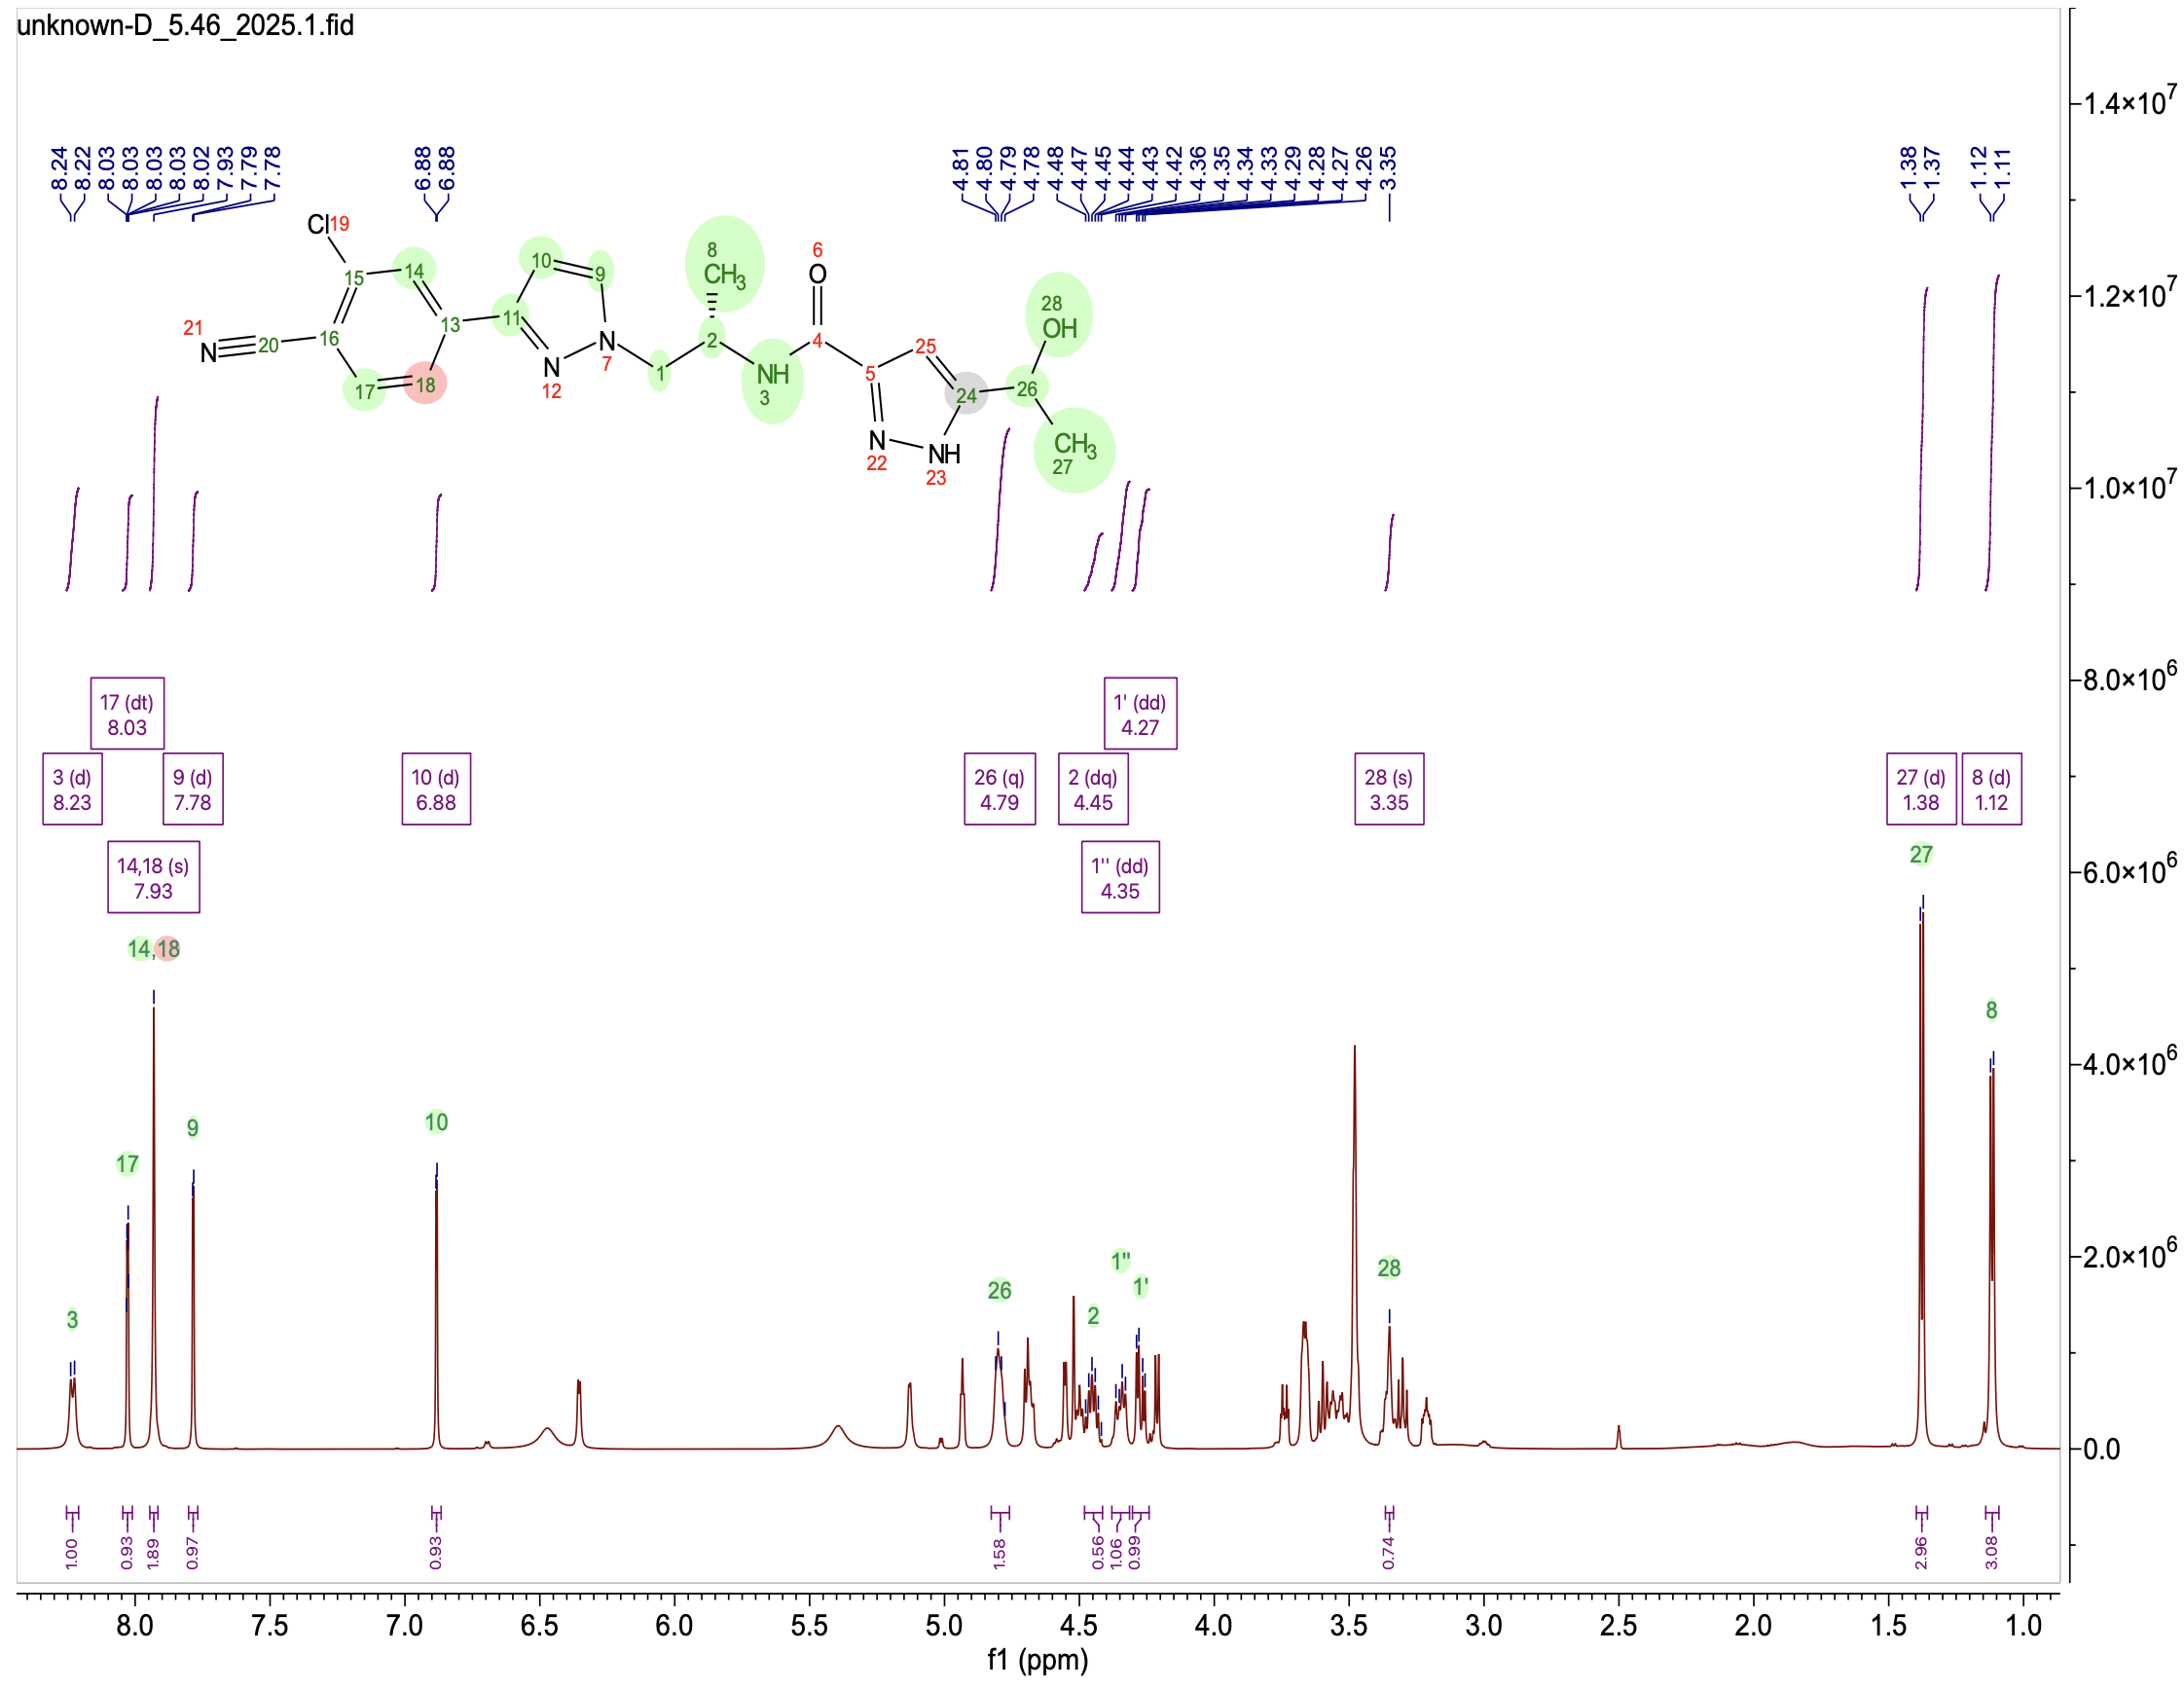
\includegraphics[width=\linewidth]{PSet3-1H.png}\\
    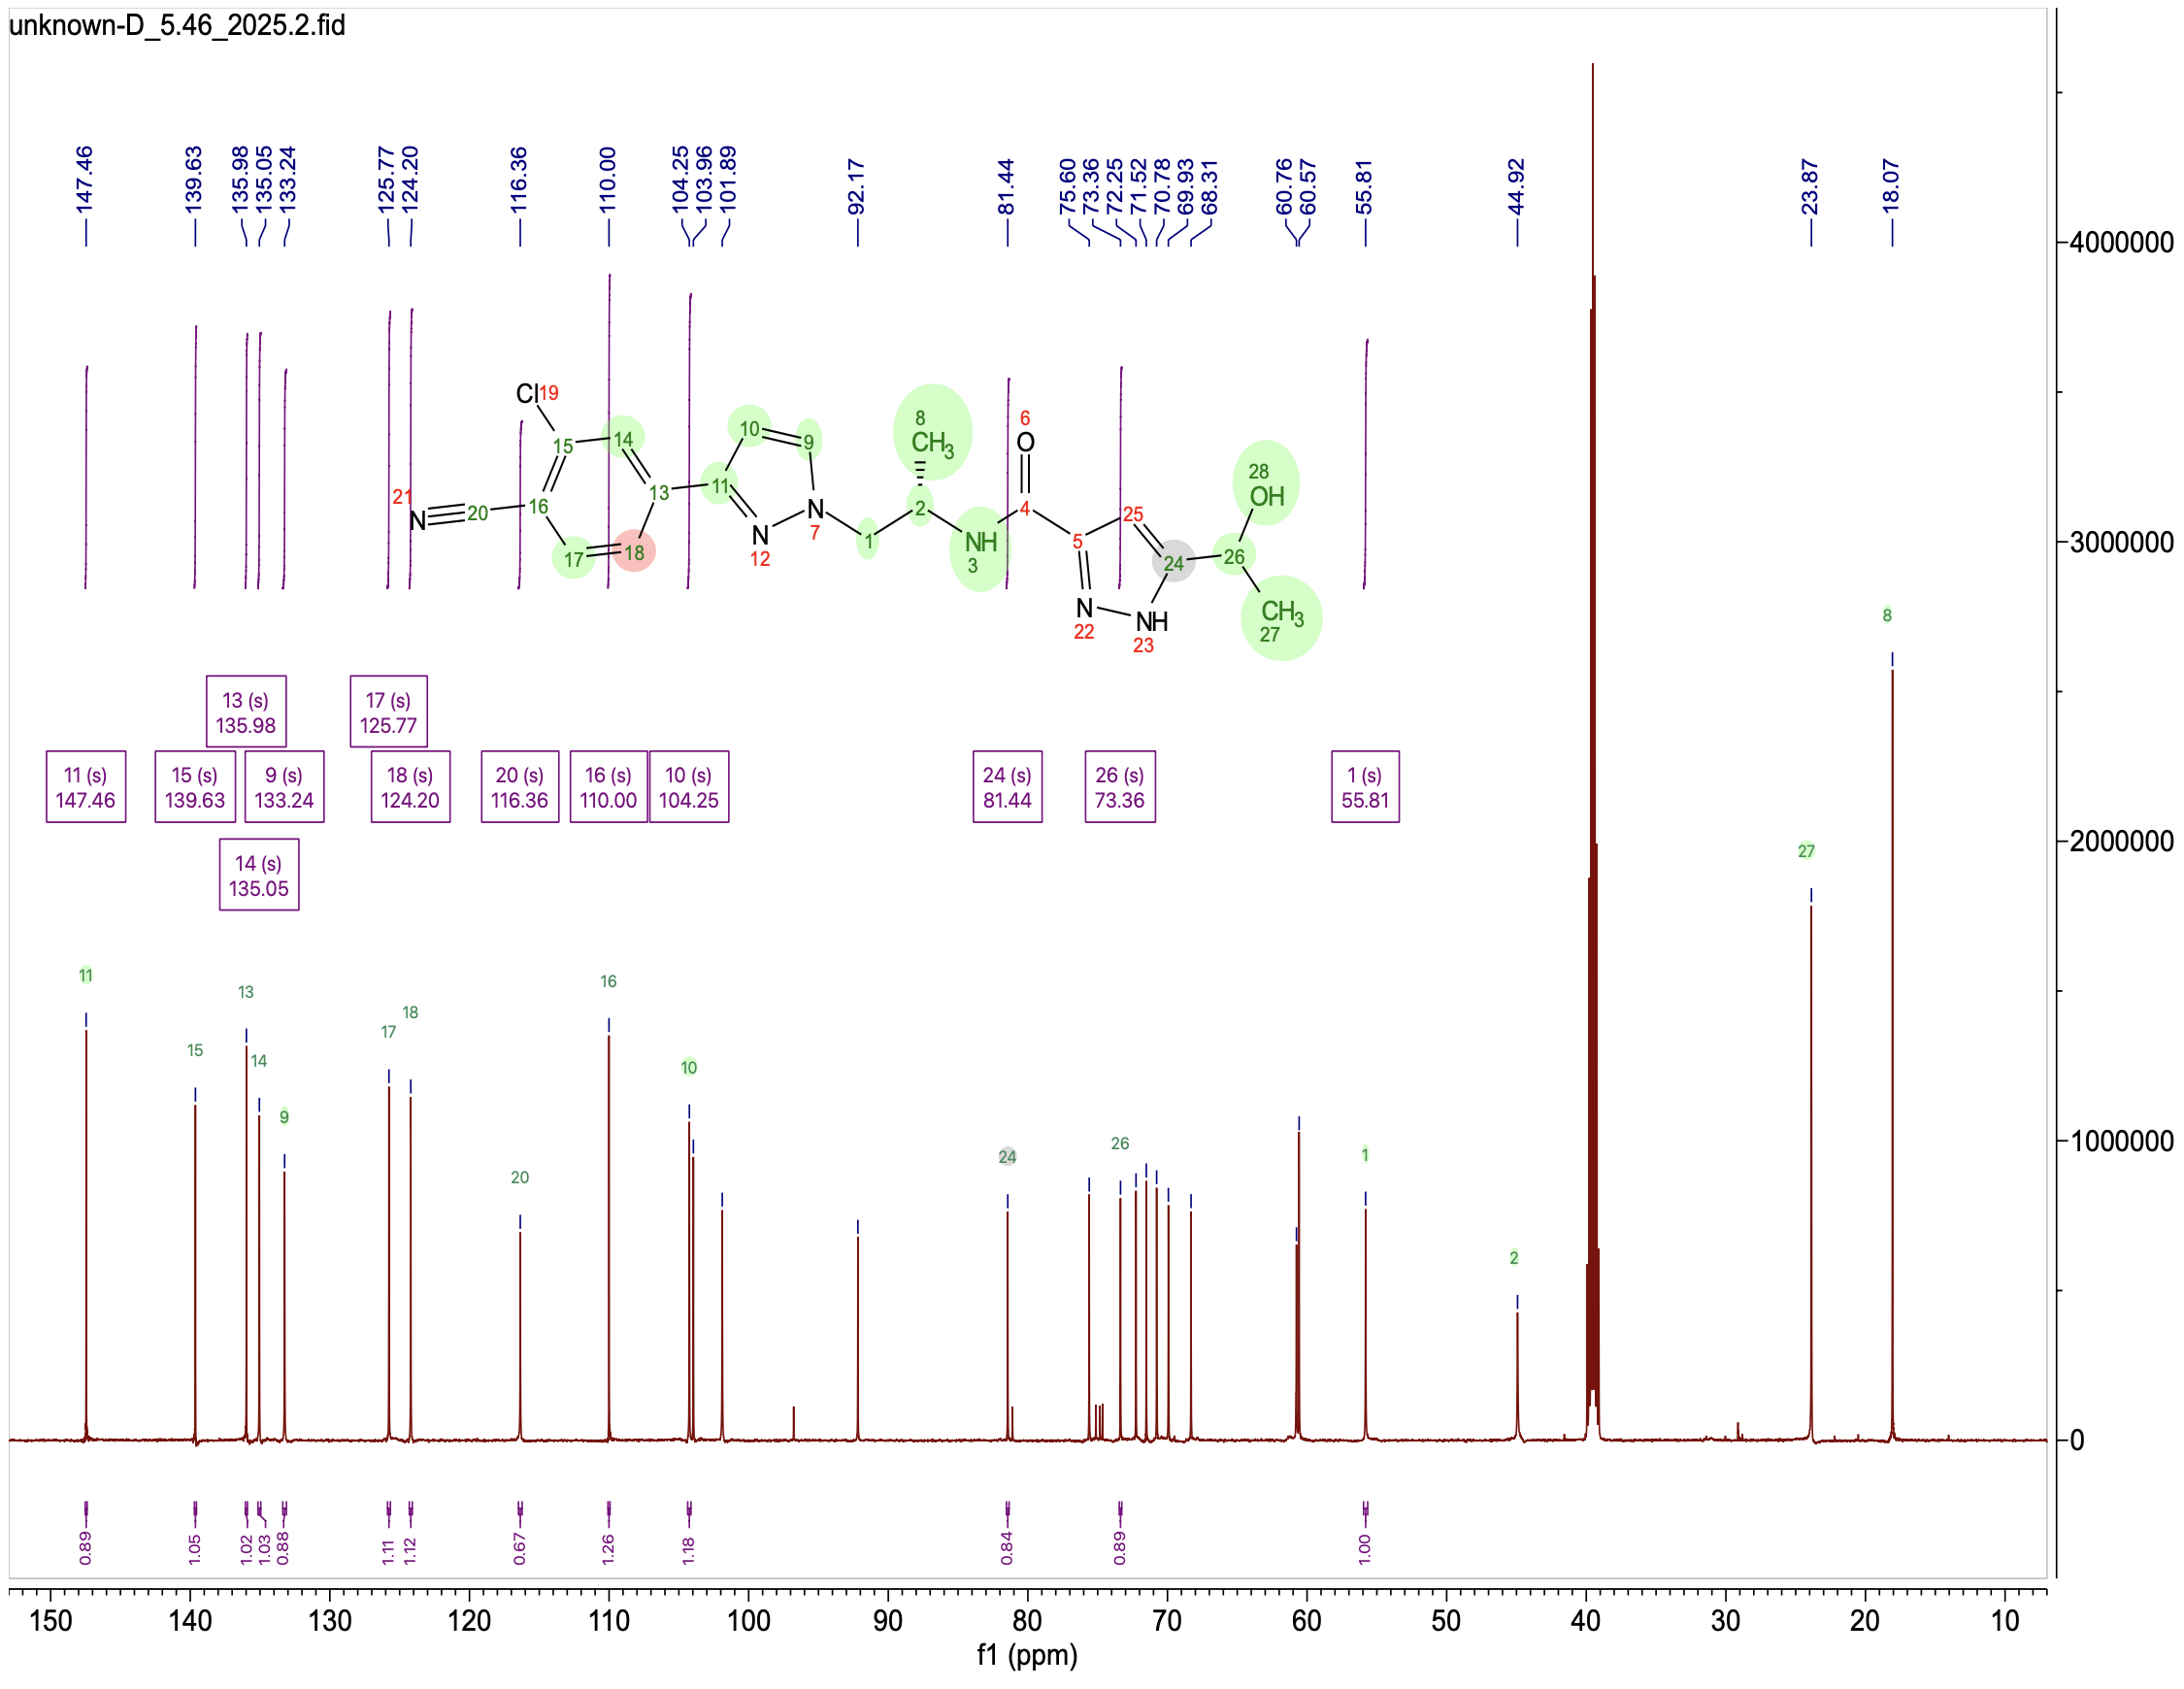
\includegraphics[width=\linewidth]{PSet3-13C.png}

    % As my analysis progressed, I encountered numerous apparent inconsistencies in the data, preventing me from achieving a full assignment. I will comment on these inconsistencies in footnotes throughout the following narrative.
\end{proof}




\end{document}